\chapter{Capitulo 7. Defectos del proceso}
\label{capitulo 3}
Debido a la complejidad inherente del proceso AFP, la aparición de defectos es inevitable durante todo el laminado. Estos defectos de fabricación pueden tener una influencia negativa significativa en el rendimiento de una estructura, por lo que es vital comprender la creación y el efecto de cada defecto. La mayoría de los defectos son un efecto secundario de la geometría de la herramienta, la dirección de la fibra y las imperfecciones del material. Todos los defectos se pueden dividir en 4 categorías principales: 

\section{Defectos de posicionamiento:}

\begin{itemize}
    \item Un Gap es cuando dos fibras adyacentes no están perfectamente colocadas uno al lado del otro y hay un espacio entre los dos. Una superposición es cuando las dos fibras adyacentes se superponen entre sí. La causa más común de espacios y superposiciones es la dirección durante el lanzamiento, ya que las fibras en un recorrido no encajan perfectamente, especialmente cuando se adopta una estrategia de cobertura paralela. Sin embargo, las lagunas y las superposiciones pueden ocurrir naturalmente fuera de la dirección si se colocan sobre una superficie de herramienta 3D compleja.

\begin{figure}[h]
    \centering
    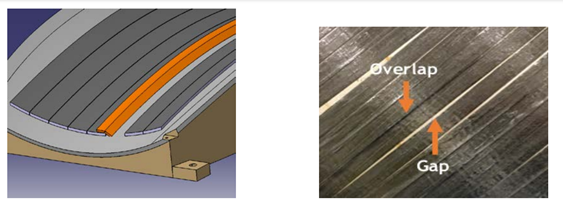
\includegraphics[width=0.9\linewidth]{eins.png}
    \caption{GAP}
    \label{fig:enter-label}
\end{figure}


\item Defectos de unión: Un Puente es cuando no se adhiere completamente a la superficie cóncava (parte hembra de la herramienta) sobre la que se depositan las fibras, dejando un espacio entre el radio de la superficie cóncava de la herramienta y la fibra. Las principales causas de un Puente son demasiada tensión. En la fibra, lo que la obligará a levantarse, o una adherencia insuficiente a la superficie que se está colocado debido a que el rodillo no proporciona contacto completo con el material del sustrato.

\begin{figure}[H]
    \centering
    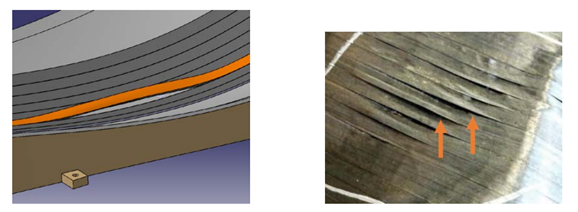
\includegraphics[width=0.9\linewidth]{zwei.png}
    \caption{Bridging}
    \label{fig:enter-label}
\end{figure}


\item Defectos de carrete: Cuando el material o el proveedor de corte unen dos cables de extremo a extremo en un carrete mediante superponiendo de 1 a 3 pulgadas entre sí y uniéndolos con tachuelas. Esto da como resultado una porción de el carrete que es más grueso que el resto y suele estar marcado con guiones blancos para su detección. En teoría, las fibras de carbono pueden tener una longitud infinita. Sin embargo, la mayoría de las AFP preimpregnadas son cintas cortadas de un rollo de cinta unidireccional de longitud finita. Estas cintas cortadas son empalmados y enrollados según las especificaciones del cliente.

\begin{figure}[H]
    \centering
    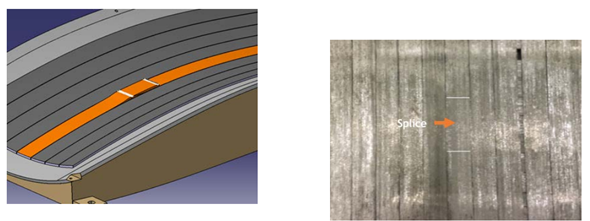
\includegraphics[width=0.9\linewidth]{drei.png}
    \caption{Splice}
    \label{fig:enter-label}
\end{figure}


\item Cuerpos extraños: Foreign object debris (FOD) se produce cuando una pequeña pieza de material compuesto, ya sea carbono “bola de pelusa” o “bola de resina” de fibra que se ha acumulado en las superficies de la cabeza u otros desechos del área de producción cae sobre la pieza durante el laminado. Esto da como resultado un pequeño exceso de volumen de material.sobre la lona si se coloca encima.

\begin{figure}[H]
    \centering
    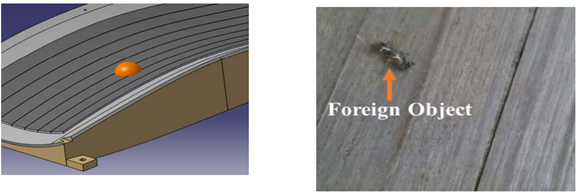
\includegraphics[width=0.9\linewidth]{vier.png}
    \caption{FOD}
    \label{fig:enter-label}
\end{figure}
\end{itemize}

En la Tabla a continuación se proporciona una lista completa de todos los tipos de defectos y sus categorías.

\begin{figure}[H]
    \centering
    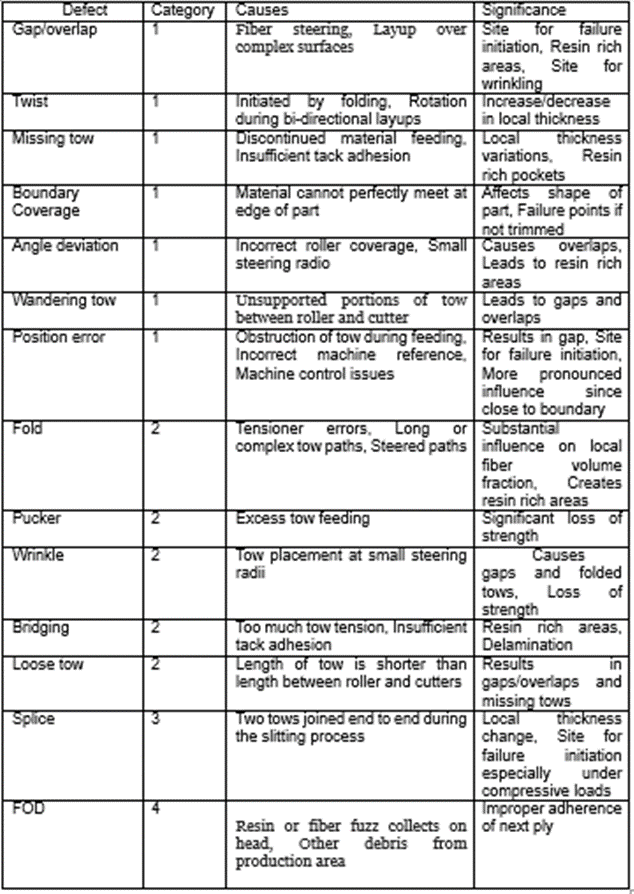
\includegraphics[width=1\linewidth]{funf.png}
    \caption{Defectos}
    \label{fig:enter-label}
\end{figure}


\textbf{}